\documentclass[1p]{elsarticle_modified}
%\bibliographystyle{elsarticle-num}

%\usepackage[colorlinks]{hyperref}
%\usepackage{abbrmath_seonhwa} %\Abb, \Ascr, \Acal ,\Abf, \Afrak
\usepackage{amsfonts}
\usepackage{amssymb}
\usepackage{amsmath}
\usepackage{amsthm}
\usepackage{scalefnt}
\usepackage{amsbsy}
\usepackage{kotex}
\usepackage{caption}
\usepackage{subfig}
\usepackage{color}
\usepackage{graphicx}
\usepackage{xcolor} %% white, black, red, green, blue, cyan, magenta, yellow
\usepackage{float}
\usepackage{setspace}
\usepackage{hyperref}

\usepackage{tikz}
\usetikzlibrary{arrows}

\usepackage{multirow}
\usepackage{array} % fixed length table
\usepackage{hhline}

%%%%%%%%%%%%%%%%%%%%%
\makeatletter
\renewcommand*\env@matrix[1][\arraystretch]{%
	\edef\arraystretch{#1}%
	\hskip -\arraycolsep
	\let\@ifnextchar\new@ifnextchar
	\array{*\c@MaxMatrixCols c}}
\makeatother %https://tex.stackexchange.com/questions/14071/how-can-i-increase-the-line-spacing-in-a-matrix
%%%%%%%%%%%%%%%

\usepackage[normalem]{ulem}

\newcommand{\msout}[1]{\ifmmode\text{\sout{\ensuremath{#1}}}\else\sout{#1}\fi}
%SOURCE: \msout is \stkout macro in https://tex.stackexchange.com/questions/20609/strikeout-in-math-mode

\newcommand{\cancel}[1]{
	\ifmmode
	{\color{red}\msout{#1}}
	\else
	{\color{red}\sout{#1}}
	\fi
}

\newcommand{\add}[1]{
	{\color{blue}\uwave{#1}}
}

\newcommand{\replace}[2]{
	\ifmmode
	{\color{red}\msout{#1}}{\color{blue}\uwave{#2}}
	\else
	{\color{red}\sout{#1}}{\color{blue}\uwave{#2}}
	\fi
}

\newcommand{\Sol}{\mathcal{S}} %segment
\newcommand{\D}{D} %diagram
\newcommand{\A}{\mathcal{A}} %arc


%%%%%%%%%%%%%%%%%%%%%%%%%%%%%5 test

\def\sl{\operatorname{\textup{SL}}(2,\Cbb)}
\def\psl{\operatorname{\textup{PSL}}(2,\Cbb)}
\def\quan{\mkern 1mu \triangleright \mkern 1mu}

\theoremstyle{definition}
\newtheorem{thm}{Theorem}[section]
\newtheorem{prop}[thm]{Proposition}
\newtheorem{lem}[thm]{Lemma}
\newtheorem{ques}[thm]{Question}
\newtheorem{cor}[thm]{Corollary}
\newtheorem{defn}[thm]{Definition}
\newtheorem{exam}[thm]{Example}
\newtheorem{rmk}[thm]{Remark}
\newtheorem{alg}[thm]{Algorithm}

\newcommand{\I}{\sqrt{-1}}
\begin{document}

%\begin{frontmatter}
%
%\title{Boundary parabolic representations of knots up to 8 crossings}
%
%%% Group authors per affiliation:
%\author{Yunhi Cho} 
%\address{Department of Mathematics, University of Seoul, Seoul, Korea}
%\ead{yhcho@uos.ac.kr}
%
%
%\author{Seonhwa Kim} %\fnref{s_kim}}
%\address{Center for Geometry and Physics, Institute for Basic Science, Pohang, 37673, Korea}
%\ead{ryeona17@ibs.re.kr}
%
%\author{Hyuk Kim}
%\address{Department of Mathematical Sciences, Seoul National University, Seoul 08826, Korea}
%\ead{hyukkim@snu.ac.kr}
%
%\author{Seokbeom Yoon}
%\address{Department of Mathematical Sciences, Seoul National University, Seoul, 08826,  Korea}
%\ead{sbyoon15@snu.ac.kr}
%
%\begin{abstract}
%We find all boundary parabolic representation of knots up to 8 crossings.
%
%\end{abstract}
%\begin{keyword}
%    \MSC[2010] 57M25 
%\end{keyword}
%
%\end{frontmatter}

%\linenumbers
%\tableofcontents
%
\newcommand\colored[1]{\textcolor{white}{\rule[-0.35ex]{0.8em}{1.4ex}}\kern-0.8em\color{red} #1}%
%\newcommand\colored[1]{\textcolor{white}{ #1}\kern-2.17ex	\textcolor{white}{ #1}\kern-1.81ex	\textcolor{white}{ #1}\kern-2.15ex\color{red}#1	}

{\Large $\underline{12a_{0920}~(K12a_{0920})}$}

\setlength{\tabcolsep}{10pt}
\renewcommand{\arraystretch}{1.6}
\vspace{1cm}\begin{tabular}{m{100pt}>{\centering\arraybackslash}m{274pt}}
\multirow{5}{120pt}{
	\centering
	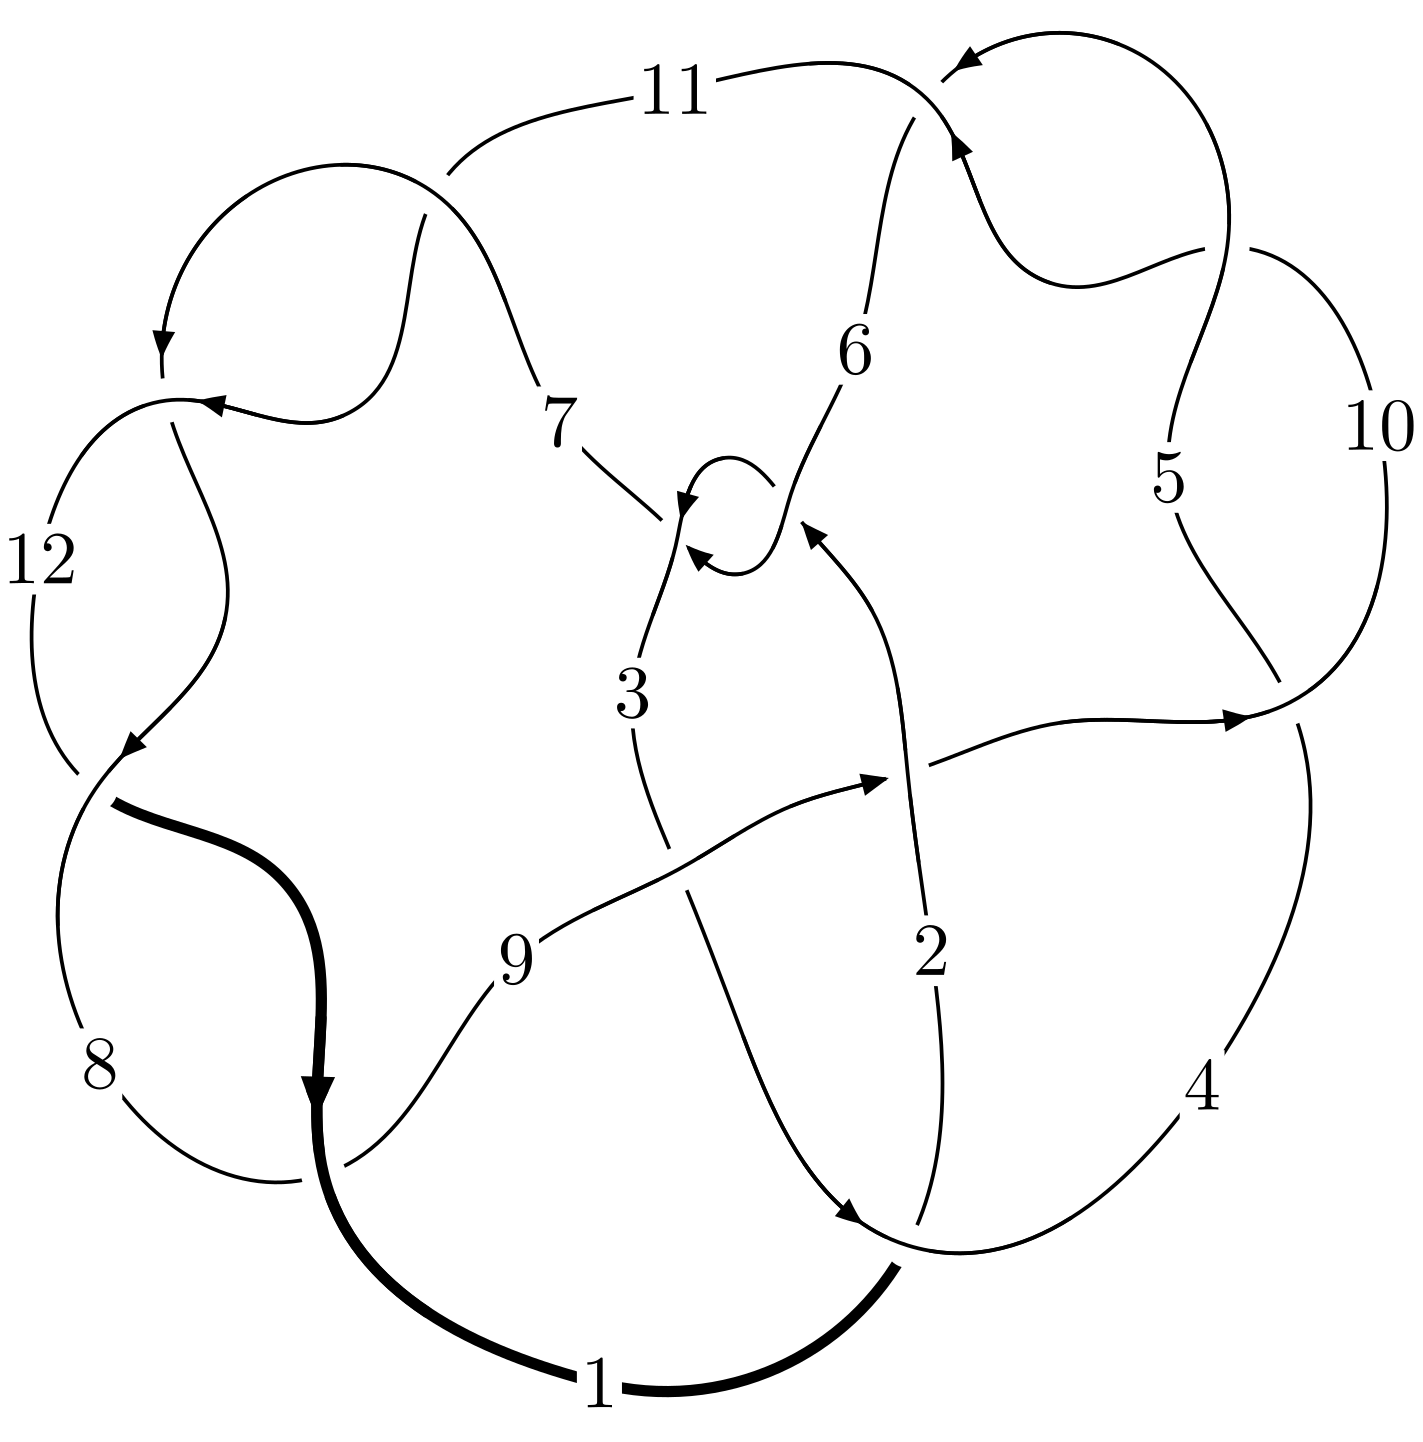
\includegraphics[width=112pt]{../../../GIT/diagram.site/Diagrams/png/1721_12a_0920.png}\\
\ \ \ A knot diagram\footnotemark}&
\allowdisplaybreaks
\textbf{Linearized knot diagam} \\
\cline{2-2}
 &
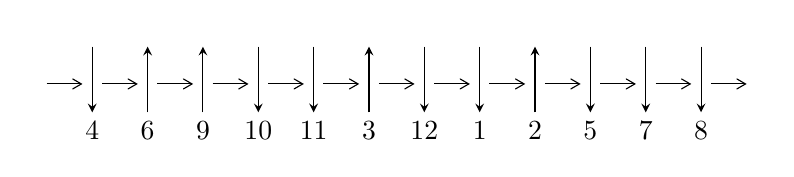
\begin{tikzpicture}[x=20pt, y=17pt]
	% nodes
	\node (C0) at (0, 0) {};
	\node (C1) at (1, 0) {};
	\node (C1U) at (1, +1) {};
	\node (C1D) at (1, -1) {4};

	\node (C2) at (2, 0) {};
	\node (C2U) at (2, +1) {};
	\node (C2D) at (2, -1) {6};

	\node (C3) at (3, 0) {};
	\node (C3U) at (3, +1) {};
	\node (C3D) at (3, -1) {9};

	\node (C4) at (4, 0) {};
	\node (C4U) at (4, +1) {};
	\node (C4D) at (4, -1) {10};

	\node (C5) at (5, 0) {};
	\node (C5U) at (5, +1) {};
	\node (C5D) at (5, -1) {11};

	\node (C6) at (6, 0) {};
	\node (C6U) at (6, +1) {};
	\node (C6D) at (6, -1) {3};

	\node (C7) at (7, 0) {};
	\node (C7U) at (7, +1) {};
	\node (C7D) at (7, -1) {12};

	\node (C8) at (8, 0) {};
	\node (C8U) at (8, +1) {};
	\node (C8D) at (8, -1) {1};

	\node (C9) at (9, 0) {};
	\node (C9U) at (9, +1) {};
	\node (C9D) at (9, -1) {2};

	\node (C10) at (10, 0) {};
	\node (C10U) at (10, +1) {};
	\node (C10D) at (10, -1) {5};

	\node (C11) at (11, 0) {};
	\node (C11U) at (11, +1) {};
	\node (C11D) at (11, -1) {7};

	\node (C12) at (12, 0) {};
	\node (C12U) at (12, +1) {};
	\node (C12D) at (12, -1) {8};
	\node (C13) at (13, 0) {};

	% arrows
	\draw[->,>={angle 60}]
	(C0) edge (C1) (C1) edge (C2) (C2) edge (C3) (C3) edge (C4) (C4) edge (C5) (C5) edge (C6) (C6) edge (C7) (C7) edge (C8) (C8) edge (C9) (C9) edge (C10) (C10) edge (C11) (C11) edge (C12) (C12) edge (C13) ;	\draw[->,>=stealth]
	(C1U) edge (C1D) (C2D) edge (C2U) (C3D) edge (C3U) (C4U) edge (C4D) (C5U) edge (C5D) (C6D) edge (C6U) (C7U) edge (C7D) (C8U) edge (C8D) (C9D) edge (C9U) (C10U) edge (C10D) (C11U) edge (C11D) (C12U) edge (C12D) ;
	\end{tikzpicture} \\
\hhline{~~} \\& 
\textbf{Solving Sequence} \\ \cline{2-2} 
 &
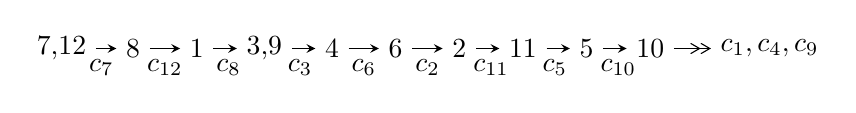
\begin{tikzpicture}[x=23pt, y=7pt]
	% node
	\node (A0) at (-1/8, 0) {7,12};
	\node (A1) at (1, 0) {8};
	\node (A2) at (2, 0) {1};
	\node (A3) at (49/16, 0) {3,9};
	\node (A4) at (33/8, 0) {4};
	\node (A5) at (41/8, 0) {6};
	\node (A6) at (49/8, 0) {2};
	\node (A7) at (57/8, 0) {11};
	\node (A8) at (65/8, 0) {5};
	\node (A9) at (73/8, 0) {10};
	\node (C1) at (1/2, -1) {$c_{7}$};
	\node (C2) at (3/2, -1) {$c_{12}$};
	\node (C3) at (5/2, -1) {$c_{8}$};
	\node (C4) at (29/8, -1) {$c_{3}$};
	\node (C5) at (37/8, -1) {$c_{6}$};
	\node (C6) at (45/8, -1) {$c_{2}$};
	\node (C7) at (53/8, -1) {$c_{11}$};
	\node (C8) at (61/8, -1) {$c_{5}$};
	\node (C9) at (69/8, -1) {$c_{10}$};
	\node (A10) at (11, 0) {$c_{1},c_{4},c_{9}$};

	% edge
	\draw[->,>=stealth]	
	(A0) edge (A1) (A1) edge (A2) (A2) edge (A3) (A3) edge (A4) (A4) edge (A5) (A5) edge (A6) (A6) edge (A7) (A7) edge (A8) (A8) edge (A9) ;
	\draw[->>,>={angle 60}]	
	(A9) edge (A10);
\end{tikzpicture} \\ 

\end{tabular} \\

\footnotetext{
The image of knot diagram is generated by the software ``\textbf{Draw programme}" developed by Andrew Bartholomew(\url{http://www.layer8.co.uk/maths/draw/index.htm\#Running-draw}), where we modified some parts for our purpose(\url{https://github.com/CATsTAILs/LinksPainter}).
}\phantom \\ \newline 
\centering \textbf{Ideals for irreducible components\footnotemark of $X_{\text{par}}$} 
 
\begin{align*}
I^u_{1}&=\langle 
5.21460\times10^{59} u^{68}-2.30775\times10^{60} u^{67}+\cdots+3.10307\times10^{59} b+1.14731\times10^{61},\\
\phantom{I^u_{1}}&\phantom{= \langle  }5.06049\times10^{60} u^{68}-2.13379\times10^{61} u^{67}+\cdots+3.10307\times10^{59} a+7.69523\times10^{61},\;u^{69}-4 u^{68}+\cdots+46 u+4\rangle \\
I^u_{2}&=\langle 
- u^{14}+10 u^{12}+u^{11}-39 u^{10}-7 u^9+75 u^8+17 u^7-75 u^6-17 u^5+39 u^4+9 u^3-10 u^2+b-5 u+1,\\
\phantom{I^u_{2}}&\phantom{= \langle  }u^{16}- u^{15}+\cdots+a+5,\;u^{17}-12 u^{15}+\cdots+2 u+1\rangle \\
I^u_{3}&=\langle 
4 a^4 u+3 a^4-8 a^3 u-6 a^3+24 a^2 u+18 a^2-32 a u+19 b-43 a-2 u-30,\\
\phantom{I^u_{3}}&\phantom{= \langle  }a^5-2 a^4+a^3 u+6 a^3-2 a^2 u-10 a^2-5 a u- a+2 u-1,\;u^2+u-1\rangle \\
\\
\end{align*}
\raggedright * 3 irreducible components of $\dim_{\mathbb{C}}=0$, with total 96 representations.\\
\footnotetext{All coefficients of polynomials are rational numbers. But the coefficients are sometimes approximated in decimal forms when there is not enough margin.}
\newpage
\renewcommand{\arraystretch}{1}
\centering \section*{I. $I^u_{1}= \langle 5.21\times10^{59} u^{68}-2.31\times10^{60} u^{67}+\cdots+3.10\times10^{59} b+1.15\times10^{61},\;5.06\times10^{60} u^{68}-2.13\times10^{61} u^{67}+\cdots+3.10\times10^{59} a+7.70\times10^{61},\;u^{69}-4 u^{68}+\cdots+46 u+4 \rangle$}
\flushleft \textbf{(i) Arc colorings}\\
\begin{tabular}{m{7pt} m{180pt} m{7pt} m{180pt} }
\flushright $a_{7}=$&$\begin{pmatrix}1\\0\end{pmatrix}$ \\
\flushright $a_{12}=$&$\begin{pmatrix}0\\u\end{pmatrix}$ \\
\flushright $a_{8}=$&$\begin{pmatrix}1\\u^2\end{pmatrix}$ \\
\flushright $a_{1}=$&$\begin{pmatrix}- u\\- u^3+u\end{pmatrix}$ \\
\flushright $a_{3}=$&$\begin{pmatrix}-16.3080 u^{68}+68.7640 u^{67}+\cdots-1888.29 u-247.988\\-1.68047 u^{68}+7.43699 u^{67}+\cdots-252.125 u-36.9734\end{pmatrix}$ \\
\flushright $a_{9}=$&$\begin{pmatrix}- u^2+1\\- u^4+2 u^2\end{pmatrix}$ \\
\flushright $a_{4}=$&$\begin{pmatrix}-15.0036 u^{68}+65.3287 u^{67}+\cdots-1927.12 u-254.936\\-0.440613 u^{68}+4.28225 u^{67}+\cdots-276.144 u-38.8034\end{pmatrix}$ \\
\flushright $a_{6}=$&$\begin{pmatrix}-4.01864 u^{68}+17.3606 u^{67}+\cdots-509.348 u-63.6386\\3.42123 u^{68}-14.2674 u^{67}+\cdots+402.460 u+56.0888\end{pmatrix}$ \\
\flushright $a_{2}=$&$\begin{pmatrix}-7.35047 u^{68}+32.8090 u^{67}+\cdots-855.578 u-94.9110\\1.71041 u^{68}-5.82409 u^{67}+\cdots+94.1801 u+14.7601\end{pmatrix}$ \\
\flushright $a_{11}=$&$\begin{pmatrix}u\\u\end{pmatrix}$ \\
\flushright $a_{5}=$&$\begin{pmatrix}-3.65619 u^{68}+15.7506 u^{67}+\cdots-453.155 u-56.1645\\3.78369 u^{68}-15.8774 u^{67}+\cdots+458.653 u+63.5629\end{pmatrix}$ \\
\flushright $a_{10}=$&$\begin{pmatrix}11.0584 u^{68}-47.9229 u^{67}+\cdots+1414.70 u+185.347\\-3.29554 u^{68}+12.6333 u^{67}+\cdots-282.187 u-38.6325\end{pmatrix}$\\&\end{tabular}
\flushleft \textbf{(ii) Obstruction class $= -1$}\\~\\
\flushleft \textbf{(iii) Cusp Shapes $= 30.0615 u^{68}-134.302 u^{67}+\cdots+4382.18 u+604.662$}\\~\\
\newpage\renewcommand{\arraystretch}{1}
\flushleft \textbf{(iv) u-Polynomials at the component}\newline \\
\begin{tabular}{m{50pt}|m{274pt}}
Crossings & \hspace{64pt}u-Polynomials at each crossing \\
\hline $$\begin{aligned}c_{1}\end{aligned}$$&$\begin{aligned}
&u^{69}-3 u^{68}+\cdots+20777 u-1427
\end{aligned}$\\
\hline $$\begin{aligned}c_{2},c_{6}\end{aligned}$$&$\begin{aligned}
&u^{69}-4 u^{68}+\cdots-15 u-1
\end{aligned}$\\
\hline $$\begin{aligned}c_{3}\end{aligned}$$&$\begin{aligned}
&u^{69}- u^{68}+\cdots-231 u+293
\end{aligned}$\\
\hline $$\begin{aligned}c_{4},c_{5},c_{10}\end{aligned}$$&$\begin{aligned}
&u^{69}+u^{68}+\cdots+26 u-1
\end{aligned}$\\
\hline $$\begin{aligned}c_{7},c_{8},c_{11}\\c_{12}\end{aligned}$$&$\begin{aligned}
&u^{69}+4 u^{68}+\cdots+46 u-4
\end{aligned}$\\
\hline $$\begin{aligned}c_{9}\end{aligned}$$&$\begin{aligned}
&u^{69}+2 u^{68}+\cdots+766 u-229
\end{aligned}$\\
\hline
\end{tabular}\\~\\
\newpage\renewcommand{\arraystretch}{1}
\flushleft \textbf{(v) Riley Polynomials at the component}\newline \\
\begin{tabular}{m{50pt}|m{274pt}}
Crossings & \hspace{64pt}Riley Polynomials at each crossing \\
\hline $$\begin{aligned}c_{1}\end{aligned}$$&$\begin{aligned}
&y^{69}-27 y^{68}+\cdots+239869243 y-2036329
\end{aligned}$\\
\hline $$\begin{aligned}c_{2},c_{6}\end{aligned}$$&$\begin{aligned}
&y^{69}-28 y^{68}+\cdots+171 y-1
\end{aligned}$\\
\hline $$\begin{aligned}c_{3}\end{aligned}$$&$\begin{aligned}
&y^{69}+13 y^{68}+\cdots-450599 y-85849
\end{aligned}$\\
\hline $$\begin{aligned}c_{4},c_{5},c_{10}\end{aligned}$$&$\begin{aligned}
&y^{69}-79 y^{68}+\cdots+462 y-1
\end{aligned}$\\
\hline $$\begin{aligned}c_{7},c_{8},c_{11}\\c_{12}\end{aligned}$$&$\begin{aligned}
&y^{69}-84 y^{68}+\cdots+684 y-16
\end{aligned}$\\
\hline $$\begin{aligned}c_{9}\end{aligned}$$&$\begin{aligned}
&y^{69}+14 y^{68}+\cdots+8302 y-52441
\end{aligned}$\\
\hline
\end{tabular}\\~\\
\newpage\flushleft \textbf{(vi) Complex Volumes and Cusp Shapes}
$$\begin{array}{c|c|c}  
\text{Solutions to }I^u_{1}& \I (\text{vol} + \sqrt{-1}CS) & \text{Cusp shape}\\
 \hline 
\begin{aligned}
u &= -0.858609 + 0.509133 I \\
a &= -0.13290 + 1.46749 I \\
b &= \phantom{-}1.119670 + 0.509880 I\end{aligned}
 & \phantom{-}0.11883 + 8.23224 I & \phantom{-0.000000 } 0 \\ \hline\begin{aligned}
u &= -0.858609 - 0.509133 I \\
a &= -0.13290 - 1.46749 I \\
b &= \phantom{-}1.119670 - 0.509880 I\end{aligned}
 & \phantom{-}0.11883 - 8.23224 I & \phantom{-0.000000 } 0 \\ \hline\begin{aligned}
u &= \phantom{-}0.922201 + 0.343620 I \\
a &= -0.226022 - 0.690778 I \\
b &= -0.396644 - 1.154280 I\end{aligned}
 & -9.14129 - 5.71438 I & \phantom{-0.000000 } 0 \\ \hline\begin{aligned}
u &= \phantom{-}0.922201 - 0.343620 I \\
a &= -0.226022 + 0.690778 I \\
b &= -0.396644 + 1.154280 I\end{aligned}
 & -9.14129 + 5.71438 I & \phantom{-0.000000 } 0 \\ \hline\begin{aligned}
u &= \phantom{-}0.957142 + 0.344138 I \\
a &= \phantom{-}0.346935 - 0.313197 I \\
b &= \phantom{-}0.956665 + 0.106533 I\end{aligned}
 & -0.408920 + 0.368294 I & \phantom{-0.000000 } 0 \\ \hline\begin{aligned}
u &= \phantom{-}0.957142 - 0.344138 I \\
a &= \phantom{-}0.346935 + 0.313197 I \\
b &= \phantom{-}0.956665 - 0.106533 I\end{aligned}
 & -0.408920 - 0.368294 I & \phantom{-0.000000 } 0 \\ \hline\begin{aligned}
u &= -0.761381 + 0.691428 I \\
a &= \phantom{-}0.903514 - 0.730666 I \\
b &= -1.019750 - 0.567692 I\end{aligned}
 & -6.72025 + 2.21455 I & \phantom{-0.000000 } 0 \\ \hline\begin{aligned}
u &= -0.761381 - 0.691428 I \\
a &= \phantom{-}0.903514 + 0.730666 I \\
b &= -1.019750 + 0.567692 I\end{aligned}
 & -6.72025 - 2.21455 I & \phantom{-0.000000 } 0 \\ \hline\begin{aligned}
u &= \phantom{-}0.875291 + 0.317279 I \\
a &= -0.65426 + 1.54098 I \\
b &= -0.941128 + 0.295855 I\end{aligned}
 & -0.11613 - 2.68304 I & \phantom{-0.000000 } 0 \\ \hline\begin{aligned}
u &= \phantom{-}0.875291 - 0.317279 I \\
a &= -0.65426 - 1.54098 I \\
b &= -0.941128 - 0.295855 I\end{aligned}
 & -0.11613 + 2.68304 I & \phantom{-0.000000 } 0\\
 \hline 
 \end{array}$$\newpage$$\begin{array}{c|c|c}  
\text{Solutions to }I^u_{1}& \I (\text{vol} + \sqrt{-1}CS) & \text{Cusp shape}\\
 \hline 
\begin{aligned}
u &= \phantom{-}0.888247 + 0.623182 I \\
a &= \phantom{-}0.428773 + 1.236830 I \\
b &= -1.198570 + 0.737599 I\end{aligned}
 & -6.69655 - 12.30450 I & \phantom{-0.000000 } 0 \\ \hline\begin{aligned}
u &= \phantom{-}0.888247 - 0.623182 I \\
a &= \phantom{-}0.428773 - 1.236830 I \\
b &= -1.198570 - 0.737599 I\end{aligned}
 & -6.69655 + 12.30450 I & \phantom{-0.000000 } 0 \\ \hline\begin{aligned}
u &= \phantom{-}0.068085 + 0.890261 I \\
a &= \phantom{-}0.549835 + 0.167489 I \\
b &= -1.014710 - 0.607088 I\end{aligned}
 & -4.19382 + 7.32485 I & \phantom{-0.000000 } 0 \\ \hline\begin{aligned}
u &= \phantom{-}0.068085 - 0.890261 I \\
a &= \phantom{-}0.549835 - 0.167489 I \\
b &= -1.014710 + 0.607088 I\end{aligned}
 & -4.19382 - 7.32485 I & \phantom{-0.000000 } 0 \\ \hline\begin{aligned}
u &= \phantom{-}0.627745 + 0.554827 I \\
a &= -0.857946 - 0.838190 I \\
b &= \phantom{-}0.676355 - 0.302159 I\end{aligned}
 & -1.22245 - 1.88994 I & \phantom{-0.000000 } 0 \\ \hline\begin{aligned}
u &= \phantom{-}0.627745 - 0.554827 I \\
a &= -0.857946 + 0.838190 I \\
b &= \phantom{-}0.676355 + 0.302159 I\end{aligned}
 & -1.22245 + 1.88994 I & \phantom{-0.000000 } 0 \\ \hline\begin{aligned}
u &= -0.751462 + 0.303115 I \\
a &= \phantom{-}0.418529 - 1.137040 I \\
b &= \phantom{-}0.165717 - 0.819333 I\end{aligned}
 & -2.66510 + 3.50831 I & -10.49360 - 7.33854 I \\ \hline\begin{aligned}
u &= -0.751462 - 0.303115 I \\
a &= \phantom{-}0.418529 + 1.137040 I \\
b &= \phantom{-}0.165717 + 0.819333 I\end{aligned}
 & -2.66510 - 3.50831 I & -10.49360 + 7.33854 I \\ \hline\begin{aligned}
u &= -1.190400 + 0.048571 I \\
a &= \phantom{-}0.888159 - 0.271946 I \\
b &= \phantom{-}0.604132 - 0.446757 I\end{aligned}
 & -7.88819 + 0.32180 I & \phantom{-0.000000 } 0 \\ \hline\begin{aligned}
u &= -1.190400 - 0.048571 I \\
a &= \phantom{-}0.888159 + 0.271946 I \\
b &= \phantom{-}0.604132 + 0.446757 I\end{aligned}
 & -7.88819 - 0.32180 I & \phantom{-0.000000 } 0\\
 \hline 
 \end{array}$$\newpage$$\begin{array}{c|c|c}  
\text{Solutions to }I^u_{1}& \I (\text{vol} + \sqrt{-1}CS) & \text{Cusp shape}\\
 \hline 
\begin{aligned}
u &= -0.747922 + 0.141109 I \\
a &= -1.18456 + 1.77018 I \\
b &= \phantom{-}1.046390 + 0.542070 I\end{aligned}
 & -6.49393 + 4.52204 I & -12.42024 - 4.96803 I \\ \hline\begin{aligned}
u &= -0.747922 - 0.141109 I \\
a &= -1.18456 - 1.77018 I \\
b &= \phantom{-}1.046390 - 0.542070 I\end{aligned}
 & -6.49393 - 4.52204 I & -12.42024 + 4.96803 I \\ \hline\begin{aligned}
u &= -0.278701 + 0.697012 I \\
a &= \phantom{-}0.918131 - 0.701090 I \\
b &= -0.633259 + 0.581048 I\end{aligned}
 & -5.39570 + 2.53481 I & -8.38084 - 2.80374 I \\ \hline\begin{aligned}
u &= -0.278701 - 0.697012 I \\
a &= \phantom{-}0.918131 + 0.701090 I \\
b &= -0.633259 - 0.581048 I\end{aligned}
 & -5.39570 - 2.53481 I & -8.38084 + 2.80374 I \\ \hline\begin{aligned}
u &= -0.034826 + 0.713110 I \\
a &= -0.706288 - 0.104021 I \\
b &= \phantom{-}1.077410 - 0.310611 I\end{aligned}
 & \phantom{-}2.61982 - 4.13722 I & -1.23735 + 6.70183 I \\ \hline\begin{aligned}
u &= -0.034826 - 0.713110 I \\
a &= -0.706288 + 0.104021 I \\
b &= \phantom{-}1.077410 + 0.310611 I\end{aligned}
 & \phantom{-}2.61982 + 4.13722 I & -1.23735 - 6.70183 I \\ \hline\begin{aligned}
u &= -1.147790 + 0.605056 I \\
a &= -0.280564 - 0.113102 I \\
b &= -0.707022 + 0.513747 I\end{aligned}
 & -7.79544 - 2.18356 I & \phantom{-0.000000 } 0 \\ \hline\begin{aligned}
u &= -1.147790 - 0.605056 I \\
a &= -0.280564 + 0.113102 I \\
b &= -0.707022 - 0.513747 I\end{aligned}
 & -7.79544 + 2.18356 I & \phantom{-0.000000 } 0 \\ \hline\begin{aligned}
u &= \phantom{-}0.549539 + 0.428722 I \\
a &= -0.92689 - 1.74841 I \\
b &= \phantom{-}1.001700 - 0.945056 I\end{aligned}
 & -3.37002 - 4.91183 I & -5.12008 + 9.10431 I \\ \hline\begin{aligned}
u &= \phantom{-}0.549539 - 0.428722 I \\
a &= -0.92689 + 1.74841 I \\
b &= \phantom{-}1.001700 + 0.945056 I\end{aligned}
 & -3.37002 + 4.91183 I & -5.12008 - 9.10431 I\\
 \hline 
 \end{array}$$\newpage$$\begin{array}{c|c|c}  
\text{Solutions to }I^u_{1}& \I (\text{vol} + \sqrt{-1}CS) & \text{Cusp shape}\\
 \hline 
\begin{aligned}
u &= -0.603111 + 0.317010 I \\
a &= -0.06954 - 1.62856 I \\
b &= -1.039670 - 0.531907 I\end{aligned}
 & \phantom{-}1.42958 + 2.33297 I & -0.70777 - 7.76145 I \\ \hline\begin{aligned}
u &= -0.603111 - 0.317010 I \\
a &= -0.06954 + 1.62856 I \\
b &= -1.039670 + 0.531907 I\end{aligned}
 & \phantom{-}1.42958 - 2.33297 I & -0.70777 + 7.76145 I \\ \hline\begin{aligned}
u &= -1.36225\phantom{ +0.000000I} \\
a &= -0.107589\phantom{ +0.000000I} \\
b &= -1.38678\phantom{ +0.000000I}\end{aligned}
 & -1.59788\phantom{ +0.000000I} & \phantom{-0.000000 } 0 \\ \hline\begin{aligned}
u &= \phantom{-}0.347963 + 0.505319 I \\
a &= \phantom{-}0.188527 - 0.656901 I \\
b &= \phantom{-}1.003340 + 0.715218 I\end{aligned}
 & -2.79726 + 1.63095 I & -4.89103 - 0.22167 I \\ \hline\begin{aligned}
u &= \phantom{-}0.347963 - 0.505319 I \\
a &= \phantom{-}0.188527 + 0.656901 I \\
b &= \phantom{-}1.003340 - 0.715218 I\end{aligned}
 & -2.79726 - 1.63095 I & -4.89103 + 0.22167 I \\ \hline\begin{aligned}
u &= -1.47026\phantom{ +0.000000I} \\
a &= \phantom{-}0.903464\phantom{ +0.000000I} \\
b &= \phantom{-}1.02182\phantom{ +0.000000I}\end{aligned}
 & -8.11663\phantom{ +0.000000I} & \phantom{-0.000000 } 0 \\ \hline\begin{aligned}
u &= \phantom{-}1.53884 + 0.08382 I \\
a &= \phantom{-}0.51726 + 1.39825 I \\
b &= -0.030549 + 0.170011 I\end{aligned}
 & -11.09110 - 4.38044 I & \phantom{-0.000000 } 0 \\ \hline\begin{aligned}
u &= \phantom{-}1.53884 - 0.08382 I \\
a &= \phantom{-}0.51726 - 1.39825 I \\
b &= -0.030549 - 0.170011 I\end{aligned}
 & -11.09110 + 4.38044 I & \phantom{-0.000000 } 0 \\ \hline\begin{aligned}
u &= \phantom{-}1.54919\phantom{ +0.000000I} \\
a &= -1.05617\phantom{ +0.000000I} \\
b &= -1.67326\phantom{ +0.000000I}\end{aligned}
 & -3.72894\phantom{ +0.000000I} & \phantom{-0.000000 } 0 \\ \hline\begin{aligned}
u &= -1.57061 + 0.09574 I \\
a &= \phantom{-}0.29032 + 2.12661 I \\
b &= \phantom{-}1.01604 + 1.19413 I\end{aligned}
 & -10.56740 + 6.67317 I & \phantom{-0.000000 } 0\\
 \hline 
 \end{array}$$\newpage$$\begin{array}{c|c|c}  
\text{Solutions to }I^u_{1}& \I (\text{vol} + \sqrt{-1}CS) & \text{Cusp shape}\\
 \hline 
\begin{aligned}
u &= -1.57061 - 0.09574 I \\
a &= \phantom{-}0.29032 - 2.12661 I \\
b &= \phantom{-}1.01604 - 1.19413 I\end{aligned}
 & -10.56740 - 6.67317 I & \phantom{-0.000000 } 0 \\ \hline\begin{aligned}
u &= \phantom{-}1.59295 + 0.06255 I \\
a &= -0.65470 + 1.63501 I \\
b &= -1.054310 + 0.900547 I\end{aligned}
 & -6.11344 - 3.58029 I & \phantom{-0.000000 } 0 \\ \hline\begin{aligned}
u &= \phantom{-}1.59295 - 0.06255 I \\
a &= -0.65470 - 1.63501 I \\
b &= -1.054310 - 0.900547 I\end{aligned}
 & -6.11344 + 3.58029 I & \phantom{-0.000000 } 0 \\ \hline\begin{aligned}
u &= -0.090552 + 0.392237 I \\
a &= \phantom{-}0.536976 - 1.059100 I \\
b &= -1.143200 + 0.046612 I\end{aligned}
 & \phantom{-}2.68421 + 0.16764 I & \phantom{-}2.41572 - 0.19332 I \\ \hline\begin{aligned}
u &= -0.090552 - 0.392237 I \\
a &= \phantom{-}0.536976 + 1.059100 I \\
b &= -1.143200 - 0.046612 I\end{aligned}
 & \phantom{-}2.68421 - 0.16764 I & \phantom{-}2.41572 + 0.19332 I \\ \hline\begin{aligned}
u &= -1.61062 + 0.16002 I \\
a &= -0.034132 + 1.263440 I \\
b &= \phantom{-}0.891494 + 0.558679 I\end{aligned}
 & -8.89500 + 4.54856 I & \phantom{-0.000000 } 0 \\ \hline\begin{aligned}
u &= -1.61062 - 0.16002 I \\
a &= -0.034132 - 1.263440 I \\
b &= \phantom{-}0.891494 - 0.558679 I\end{aligned}
 & -8.89500 - 4.54856 I & \phantom{-0.000000 } 0 \\ \hline\begin{aligned}
u &= \phantom{-}0.070878 + 0.373596 I \\
a &= -0.958588 + 0.155139 I \\
b &= -0.002941 + 0.459481 I\end{aligned}
 & -0.359603 - 1.131530 I & -5.56898 + 5.13888 I \\ \hline\begin{aligned}
u &= \phantom{-}0.070878 - 0.373596 I \\
a &= -0.958588 - 0.155139 I \\
b &= -0.002941 - 0.459481 I\end{aligned}
 & -0.359603 + 1.131530 I & -5.56898 - 5.13888 I \\ \hline\begin{aligned}
u &= \phantom{-}1.62259 + 0.07416 I \\
a &= \phantom{-}0.41905 + 1.55527 I \\
b &= \phantom{-}0.337200 + 0.935815 I\end{aligned}
 & -10.84000 - 4.89494 I & \phantom{-0.000000 } 0\\
 \hline 
 \end{array}$$\newpage$$\begin{array}{c|c|c}  
\text{Solutions to }I^u_{1}& \I (\text{vol} + \sqrt{-1}CS) & \text{Cusp shape}\\
 \hline 
\begin{aligned}
u &= \phantom{-}1.62259 - 0.07416 I \\
a &= \phantom{-}0.41905 - 1.55527 I \\
b &= \phantom{-}0.337200 - 0.935815 I\end{aligned}
 & -10.84000 + 4.89494 I & \phantom{-0.000000 } 0 \\ \hline\begin{aligned}
u &= \phantom{-}1.64324 + 0.03991 I \\
a &= \phantom{-}0.106947 - 1.306450 I \\
b &= \phantom{-}1.29168 - 0.59412 I\end{aligned}
 & -14.8905 - 5.2157 I & \phantom{-0.000000 } 0 \\ \hline\begin{aligned}
u &= \phantom{-}1.64324 - 0.03991 I \\
a &= \phantom{-}0.106947 + 1.306450 I \\
b &= \phantom{-}1.29168 + 0.59412 I\end{aligned}
 & -14.8905 + 5.2157 I & \phantom{-0.000000 } 0 \\ \hline\begin{aligned}
u &= \phantom{-}1.66632 + 0.14638 I \\
a &= \phantom{-}0.46733 - 1.56172 I \\
b &= \phantom{-}1.147590 - 0.686553 I\end{aligned}
 & -8.56853 - 10.77570 I & \phantom{-0.000000 } 0 \\ \hline\begin{aligned}
u &= \phantom{-}1.66632 - 0.14638 I \\
a &= \phantom{-}0.46733 + 1.56172 I \\
b &= \phantom{-}1.147590 + 0.686553 I\end{aligned}
 & -8.56853 + 10.77570 I & \phantom{-0.000000 } 0 \\ \hline\begin{aligned}
u &= -1.67496 + 0.09834 I \\
a &= -0.51698 + 1.53291 I \\
b &= -0.50081 + 1.47766 I\end{aligned}
 & -18.1559 + 7.4706 I & \phantom{-0.000000 } 0 \\ \hline\begin{aligned}
u &= -1.67496 - 0.09834 I \\
a &= -0.51698 - 1.53291 I \\
b &= -0.50081 - 1.47766 I\end{aligned}
 & -18.1559 - 7.4706 I & \phantom{-0.000000 } 0 \\ \hline\begin{aligned}
u &= \phantom{-}1.66700 + 0.20966 I \\
a &= -0.097293 + 1.135820 I \\
b &= -1.29837 + 0.61433 I\end{aligned}
 & -15.0060 - 5.7097 I & \phantom{-0.000000 } 0 \\ \hline\begin{aligned}
u &= \phantom{-}1.66700 - 0.20966 I \\
a &= -0.097293 - 1.135820 I \\
b &= -1.29837 - 0.61433 I\end{aligned}
 & -15.0060 + 5.7097 I & \phantom{-0.000000 } 0 \\ \hline\begin{aligned}
u &= -1.67919 + 0.09590 I \\
a &= -0.70802 - 1.36350 I \\
b &= -0.843032 - 0.540808 I\end{aligned}
 & -9.07614 + 4.33421 I & \phantom{-0.000000 } 0\\
 \hline 
 \end{array}$$\newpage$$\begin{array}{c|c|c}  
\text{Solutions to }I^u_{1}& \I (\text{vol} + \sqrt{-1}CS) & \text{Cusp shape}\\
 \hline 
\begin{aligned}
u &= -1.67919 - 0.09590 I \\
a &= -0.70802 + 1.36350 I \\
b &= -0.843032 + 0.540808 I\end{aligned}
 & -9.07614 - 4.33421 I & \phantom{-0.000000 } 0 \\ \hline\begin{aligned}
u &= -1.67662 + 0.18420 I \\
a &= -0.33035 - 1.57967 I \\
b &= -1.32832 - 0.86095 I\end{aligned}
 & -15.4447 + 15.4584 I & \phantom{-0.000000 } 0 \\ \hline\begin{aligned}
u &= -1.67662 - 0.18420 I \\
a &= -0.33035 + 1.57967 I \\
b &= -1.32832 + 0.86095 I\end{aligned}
 & -15.4447 - 15.4584 I & \phantom{-0.000000 } 0 \\ \hline\begin{aligned}
u &= -0.257782 + 0.029613 I \\
a &= \phantom{-}3.42531 + 5.22024 I \\
b &= \phantom{-}0.515844 - 0.457634 I\end{aligned}
 & -4.89351 - 3.67092 I & -12.31151 - 0.80644 I \\ \hline\begin{aligned}
u &= -0.257782 - 0.029613 I \\
a &= \phantom{-}3.42531 - 5.22024 I \\
b &= \phantom{-}0.515844 + 0.457634 I\end{aligned}
 & -4.89351 + 3.67092 I & -12.31151 + 0.80644 I \\ \hline\begin{aligned}
u &= \phantom{-}1.74045 + 0.06218 I \\
a &= \phantom{-}0.068694 - 0.932107 I \\
b &= -0.032884 - 0.887424 I\end{aligned}
 & -18.5613 - 0.1635 I & \phantom{-0.000000 } 0 \\ \hline\begin{aligned}
u &= \phantom{-}1.74045 - 0.06218 I \\
a &= \phantom{-}0.068694 + 0.932107 I \\
b &= -0.032884 + 0.887424 I\end{aligned}
 & -18.5613 + 0.1635 I & \phantom{-0.000000 } 0 \\ \hline\begin{aligned}
u &= -0.222069\phantom{ +0.000000I} \\
a &= -1.80233\phantom{ +0.000000I} \\
b &= -1.36002\phantom{ +0.000000I}\end{aligned}
 & \phantom{-}2.83320\phantom{ +0.000000I} & \phantom{-}10.8910\phantom{ +0.000000I} \\ \hline\begin{aligned}
u &= \phantom{-}1.81750\phantom{ +0.000000I} \\
a &= \phantom{-}0.292085\phantom{ +0.000000I} \\
b &= \phantom{-}0.0660849\phantom{ +0.000000I}\end{aligned}
 & -19.0700\phantom{ +0.000000I} & \phantom{-0.000000 } 0\\
 \hline 
 \end{array}$$\newpage\newpage\renewcommand{\arraystretch}{1}
\centering \section*{II. $I^u_{2}= \langle - u^{14}+10 u^{12}+\cdots+b+1,\;u^{16}- u^{15}+\cdots+a+5,\;u^{17}-12 u^{15}+\cdots+2 u+1 \rangle$}
\flushleft \textbf{(i) Arc colorings}\\
\begin{tabular}{m{7pt} m{180pt} m{7pt} m{180pt} }
\flushright $a_{7}=$&$\begin{pmatrix}1\\0\end{pmatrix}$ \\
\flushright $a_{12}=$&$\begin{pmatrix}0\\u\end{pmatrix}$ \\
\flushright $a_{8}=$&$\begin{pmatrix}1\\u^2\end{pmatrix}$ \\
\flushright $a_{1}=$&$\begin{pmatrix}- u\\- u^3+u\end{pmatrix}$ \\
\flushright $a_{3}=$&$\begin{pmatrix}- u^{16}+u^{15}+\cdots+2 u-5\\u^{14}-10 u^{12}+\cdots+5 u-1\end{pmatrix}$ \\
\flushright $a_{9}=$&$\begin{pmatrix}- u^2+1\\- u^4+2 u^2\end{pmatrix}$ \\
\flushright $a_{4}=$&$\begin{pmatrix}- u^{16}+u^{15}+\cdots+5 u-5\\2 u^{14}-19 u^{12}+\cdots+6 u-1\end{pmatrix}$ \\
\flushright $a_{6}=$&$\begin{pmatrix}2 u^{16}-2 u^{15}+\cdots-5 u+8\\- u^{15}- u^{14}+\cdots+u+4\end{pmatrix}$ \\
\flushright $a_{2}=$&$\begin{pmatrix}u^{16}-2 u^{15}+\cdots-10 u+7\\- u^{15}-3 u^{14}+\cdots-5 u+3\end{pmatrix}$ \\
\flushright $a_{11}=$&$\begin{pmatrix}u\\u\end{pmatrix}$ \\
\flushright $a_{5}=$&$\begin{pmatrix}2 u^{16}- u^{15}+\cdots-5 u+7\\u^{12}- u^{11}+\cdots+u+3\end{pmatrix}$ \\
\flushright $a_{10}=$&$\begin{pmatrix}-3 u^{16}+34 u^{14}+\cdots+12 u-8\\-2 u^{16}+22 u^{14}+\cdots+2 u-4\end{pmatrix}$\\&\end{tabular}
\flushleft \textbf{(ii) Obstruction class $= 1$}\\~\\
\flushleft \textbf{(iii) Cusp Shapes $= 6 u^{16}-2 u^{15}-73 u^{14}+15 u^{13}+361 u^{12}-34 u^{11}-928 u^{10}+8 u^9+1320 u^8+54 u^7-1027 u^6-59 u^5+406 u^4+53 u^3-66 u^2-38 u-4$}\\~\\
\newpage\renewcommand{\arraystretch}{1}
\flushleft \textbf{(iv) u-Polynomials at the component}\newline \\
\begin{tabular}{m{50pt}|m{274pt}}
Crossings & \hspace{64pt}u-Polynomials at each crossing \\
\hline $$\begin{aligned}c_{1}\end{aligned}$$&$\begin{aligned}
&u^{17}-6 u^{15}+\cdots+3 u-1
\end{aligned}$\\
\hline $$\begin{aligned}c_{2}\end{aligned}$$&$\begin{aligned}
&u^{17}-3 u^{16}+\cdots-3 u+1
\end{aligned}$\\
\hline $$\begin{aligned}c_{3}\end{aligned}$$&$\begin{aligned}
&u^{17}-2 u^{14}+\cdots+u+1
\end{aligned}$\\
\hline $$\begin{aligned}c_{4},c_{5}\end{aligned}$$&$\begin{aligned}
&u^{17}-10 u^{15}+\cdots+2 u-1
\end{aligned}$\\
\hline $$\begin{aligned}c_{6}\end{aligned}$$&$\begin{aligned}
&u^{17}+3 u^{16}+\cdots-3 u-1
\end{aligned}$\\
\hline $$\begin{aligned}c_{7},c_{8}\end{aligned}$$&$\begin{aligned}
&u^{17}-12 u^{15}+\cdots+2 u+1
\end{aligned}$\\
\hline $$\begin{aligned}c_{9}\end{aligned}$$&$\begin{aligned}
&u^{17}+u^{16}+\cdots-2 u^3+1
\end{aligned}$\\
\hline $$\begin{aligned}c_{10}\end{aligned}$$&$\begin{aligned}
&u^{17}-10 u^{15}+\cdots+2 u+1
\end{aligned}$\\
\hline $$\begin{aligned}c_{11},c_{12}\end{aligned}$$&$\begin{aligned}
&u^{17}-12 u^{15}+\cdots+2 u-1
\end{aligned}$\\
\hline
\end{tabular}\\~\\
\newpage\renewcommand{\arraystretch}{1}
\flushleft \textbf{(v) Riley Polynomials at the component}\newline \\
\begin{tabular}{m{50pt}|m{274pt}}
Crossings & \hspace{64pt}Riley Polynomials at each crossing \\
\hline $$\begin{aligned}c_{1}\end{aligned}$$&$\begin{aligned}
&y^{17}-12 y^{16}+\cdots+21 y-1
\end{aligned}$\\
\hline $$\begin{aligned}c_{2},c_{6}\end{aligned}$$&$\begin{aligned}
&y^{17}-17 y^{16}+\cdots+17 y-1
\end{aligned}$\\
\hline $$\begin{aligned}c_{3}\end{aligned}$$&$\begin{aligned}
&y^{17}-6 y^{15}+\cdots+3 y-1
\end{aligned}$\\
\hline $$\begin{aligned}c_{4},c_{5},c_{10}\end{aligned}$$&$\begin{aligned}
&y^{17}-20 y^{16}+\cdots+16 y-1
\end{aligned}$\\
\hline $$\begin{aligned}c_{7},c_{8},c_{11}\\c_{12}\end{aligned}$$&$\begin{aligned}
&y^{17}-24 y^{16}+\cdots+24 y-1
\end{aligned}$\\
\hline $$\begin{aligned}c_{9}\end{aligned}$$&$\begin{aligned}
&y^{17}-3 y^{16}+\cdots+6 y^2-1
\end{aligned}$\\
\hline
\end{tabular}\\~\\
\newpage\flushleft \textbf{(vi) Complex Volumes and Cusp Shapes}
$$\begin{array}{c|c|c}  
\text{Solutions to }I^u_{2}& \I (\text{vol} + \sqrt{-1}CS) & \text{Cusp shape}\\
 \hline 
\begin{aligned}
u &= \phantom{-}1.09578\phantom{ +0.000000I} \\
a &= \phantom{-}0.547612\phantom{ +0.000000I} \\
b &= \phantom{-}1.14178\phantom{ +0.000000I}\end{aligned}
 & \phantom{-}0.341936\phantom{ +0.000000I} & \phantom{-}0.875270\phantom{ +0.000000I} \\ \hline\begin{aligned}
u &= -1.123960 + 0.382204 I \\
a &= -0.478136 - 0.578939 I \\
b &= -0.617479 + 0.293759 I\end{aligned}
 & -7.13101 - 1.62524 I & -6.68084 + 0.62023 I \\ \hline\begin{aligned}
u &= -1.123960 - 0.382204 I \\
a &= -0.478136 + 0.578939 I \\
b &= -0.617479 - 0.293759 I\end{aligned}
 & -7.13101 + 1.62524 I & -6.68084 - 0.62023 I \\ \hline\begin{aligned}
u &= -1.18833\phantom{ +0.000000I} \\
a &= \phantom{-}0.0332715\phantom{ +0.000000I} \\
b &= -1.43147\phantom{ +0.000000I}\end{aligned}
 & -3.07503\phantom{ +0.000000I} & -11.9270\phantom{ +0.000000I} \\ \hline\begin{aligned}
u &= \phantom{-}0.667353 + 0.370935 I \\
a &= -0.47830 - 1.61454 I \\
b &= \phantom{-}0.724488 - 0.164054 I\end{aligned}
 & -0.59938 - 1.32532 I & -5.05705 + 2.80405 I \\ \hline\begin{aligned}
u &= \phantom{-}0.667353 - 0.370935 I \\
a &= -0.47830 + 1.61454 I \\
b &= \phantom{-}0.724488 + 0.164054 I\end{aligned}
 & -0.59938 + 1.32532 I & -5.05705 - 2.80405 I \\ \hline\begin{aligned}
u &= -0.369667 + 0.360033 I \\
a &= \phantom{-}2.85434 - 1.27851 I \\
b &= -0.773403 - 0.575136 I\end{aligned}
 & -4.67731 + 4.33112 I & -8.36560 - 8.69813 I \\ \hline\begin{aligned}
u &= -0.369667 - 0.360033 I \\
a &= \phantom{-}2.85434 + 1.27851 I \\
b &= -0.773403 + 0.575136 I\end{aligned}
 & -4.67731 - 4.33112 I & -8.36560 + 8.69813 I \\ \hline\begin{aligned}
u &= \phantom{-}1.53432\phantom{ +0.000000I} \\
a &= -1.73698\phantom{ +0.000000I} \\
b &= -1.84039\phantom{ +0.000000I}\end{aligned}
 & -6.74002\phantom{ +0.000000I} & -3.61890\phantom{ +0.000000I} \\ \hline\begin{aligned}
u &= -1.55322\phantom{ +0.000000I} \\
a &= \phantom{-}0.672900\phantom{ +0.000000I} \\
b &= \phantom{-}1.56084\phantom{ +0.000000I}\end{aligned}
 & -4.27815\phantom{ +0.000000I} & -13.1180\phantom{ +0.000000I}\\
 \hline 
 \end{array}$$\newpage$$\begin{array}{c|c|c}  
\text{Solutions to }I^u_{2}& \I (\text{vol} + \sqrt{-1}CS) & \text{Cusp shape}\\
 \hline 
\begin{aligned}
u &= \phantom{-}1.55960 + 0.10540 I \\
a &= \phantom{-}0.20362 + 1.87120 I \\
b &= -0.891995 + 0.798543 I\end{aligned}
 & -11.47150 - 5.99192 I & -13.12352 + 4.84870 I \\ \hline\begin{aligned}
u &= \phantom{-}1.55960 - 0.10540 I \\
a &= \phantom{-}0.20362 - 1.87120 I \\
b &= -0.891995 - 0.798543 I\end{aligned}
 & -11.47150 + 5.99192 I & -13.12352 - 4.84870 I \\ \hline\begin{aligned}
u &= \phantom{-}0.389234\phantom{ +0.000000I} \\
a &= -0.308648\phantom{ +0.000000I} \\
b &= \phantom{-}1.38986\phantom{ +0.000000I}\end{aligned}
 & \phantom{-}2.56515\phantom{ +0.000000I} & -19.7450\phantom{ +0.000000I} \\ \hline\begin{aligned}
u &= -1.63154 + 0.11334 I \\
a &= \phantom{-}0.255071 + 1.300460 I \\
b &= \phantom{-}0.681332 + 0.453515 I\end{aligned}
 & -8.67576 + 3.16393 I & -7.87236 - 0.20715 I \\ \hline\begin{aligned}
u &= -1.63154 - 0.11334 I \\
a &= \phantom{-}0.255071 - 1.300460 I \\
b &= \phantom{-}0.681332 - 0.453515 I\end{aligned}
 & -8.67576 - 3.16393 I & -7.87236 + 0.20715 I \\ \hline\begin{aligned}
u &= -0.315662\phantom{ +0.000000I} \\
a &= -3.47084\phantom{ +0.000000I} \\
b &= -1.66703\phantom{ +0.000000I}\end{aligned}
 & -0.212009\phantom{ +0.000000I} & \phantom{-}3.05600\phantom{ +0.000000I} \\ \hline\begin{aligned}
u &= \phantom{-}1.83431\phantom{ +0.000000I} \\
a &= -0.450508\phantom{ +0.000000I} \\
b &= -0.399475\phantom{ +0.000000I}\end{aligned}
 & -18.8982\phantom{ +0.000000I} & \phantom{-}15.6760\phantom{ +0.000000I}\\
 \hline 
 \end{array}$$\newpage\newpage\renewcommand{\arraystretch}{1}
\centering \section*{III. $I^u_{3}= \langle 4 a^4 u-8 a^3 u+\cdots-43 a-30,\;a^3 u-2 a^2 u+\cdots- a-1,\;u^2+u-1 \rangle$}
\flushleft \textbf{(i) Arc colorings}\\
\begin{tabular}{m{7pt} m{180pt} m{7pt} m{180pt} }
\flushright $a_{7}=$&$\begin{pmatrix}1\\0\end{pmatrix}$ \\
\flushright $a_{12}=$&$\begin{pmatrix}0\\u\end{pmatrix}$ \\
\flushright $a_{8}=$&$\begin{pmatrix}1\\- u+1\end{pmatrix}$ \\
\flushright $a_{1}=$&$\begin{pmatrix}- u\\- u+1\end{pmatrix}$ \\
\flushright $a_{3}=$&$\begin{pmatrix}a\\-0.210526 a^{4} u+0.421053 a^{3} u+\cdots+2.26316 a+1.57895\end{pmatrix}$ \\
\flushright $a_{9}=$&$\begin{pmatrix}u\\u\end{pmatrix}$ \\
\flushright $a_{4}=$&$\begin{pmatrix}-0.263158 a^{4} u+0.526316 a^{3} u+\cdots+0.578947 a+1.47368\\-0.473684 a^{4} u+0.947368 a^{3} u+\cdots+1.84211 a+3.05263\end{pmatrix}$ \\
\flushright $a_{6}=$&$\begin{pmatrix}-0.0526316 a^{3} u-0.315789 a^{2} u+\cdots+0.368421 a+1.26316\\-0.421053 a^{4} u+0.526316 a^{3} u+\cdots+4.73684 a+2.73684\end{pmatrix}$ \\
\flushright $a_{2}=$&$\begin{pmatrix}0.526316 a^{4} u-0.421053 a^{3} u+\cdots-1.57895 a-2.10526\\0.947368 a^{4} u-a^{3} u+\cdots-5.94737 a-3.57895\end{pmatrix}$ \\
\flushright $a_{11}=$&$\begin{pmatrix}u\\u\end{pmatrix}$ \\
\flushright $a_{5}=$&$\begin{pmatrix}-0.526316 a^{4} u+0.421053 a^{3} u+\cdots+1.57895 a+2.10526\\-0.947368 a^{4} u+a^{3} u+\cdots+5.94737 a+3.57895\end{pmatrix}$ \\
\flushright $a_{10}=$&$\begin{pmatrix}-0.473684 a^{4} u+0.315789 a^{3} u+\cdots-5.73684 a+0.210526\\-0.315789 a^{4} u+0.315789 a^{2} u+\cdots-9.68421 a-1.47368\end{pmatrix}$\\&\end{tabular}
\flushleft \textbf{(ii) Obstruction class $= -1$}\\~\\
\flushleft \textbf{(iii) Cusp Shapes $= -10$}\\~\\
\newpage\renewcommand{\arraystretch}{1}
\flushleft \textbf{(iv) u-Polynomials at the component}\newline \\
\begin{tabular}{m{50pt}|m{274pt}}
Crossings & \hspace{64pt}u-Polynomials at each crossing \\
\hline $$\begin{aligned}c_{1}\end{aligned}$$&$\begin{aligned}
&u^{10}-4 u^9+2 u^8+8 u^7-5 u^6-11 u^5+8 u^4+7 u^3-5 u^2-3 u+1
\end{aligned}$\\
\hline $$\begin{aligned}c_{2},c_{6}\end{aligned}$$&$\begin{aligned}
&u^{10}+4 u^9+2 u^8-8 u^7-5 u^6+11 u^5+8 u^4-7 u^3-5 u^2+3 u+1
\end{aligned}$\\
\hline $$\begin{aligned}c_{3}\end{aligned}$$&$\begin{aligned}
&u^{10}+2 u^8-4 u^7+5 u^6-7 u^5-12 u^4+9 u^3-5 u^2- u+1
\end{aligned}$\\
\hline $$\begin{aligned}c_{4},c_{5},c_{9}\\c_{10}\end{aligned}$$&$\begin{aligned}
&u^{10}-2 u^8- u^6+u^5+2 u^4- u^3+u^2- u-1
\end{aligned}$\\
\hline $$\begin{aligned}c_{7},c_{8},c_{11}\\c_{12}\end{aligned}$$&$\begin{aligned}
&(u^2- u-1)^5
\end{aligned}$\\
\hline
\end{tabular}\\~\\
\newpage\renewcommand{\arraystretch}{1}
\flushleft \textbf{(v) Riley Polynomials at the component}\newline \\
\begin{tabular}{m{50pt}|m{274pt}}
Crossings & \hspace{64pt}Riley Polynomials at each crossing \\
\hline $$\begin{aligned}c_{1},c_{2},c_{6}\end{aligned}$$&$\begin{aligned}
&y^{10}-12 y^9+\cdots-19 y+1
\end{aligned}$\\
\hline $$\begin{aligned}c_{3}\end{aligned}$$&$\begin{aligned}
&y^{10}+4 y^9+\cdots-11 y+1
\end{aligned}$\\
\hline $$\begin{aligned}c_{4},c_{5},c_{9}\\c_{10}\end{aligned}$$&$\begin{aligned}
&y^{10}-4 y^9+2 y^8+8 y^7-5 y^6-11 y^5+8 y^4+7 y^3-5 y^2-3 y+1
\end{aligned}$\\
\hline $$\begin{aligned}c_{7},c_{8},c_{11}\\c_{12}\end{aligned}$$&$\begin{aligned}
&(y^2-3 y+1)^5
\end{aligned}$\\
\hline
\end{tabular}\\~\\
\newpage\flushleft \textbf{(vi) Complex Volumes and Cusp Shapes}
$$\begin{array}{c|c|c}  
\text{Solutions to }I^u_{3}& \I (\text{vol} + \sqrt{-1}CS) & \text{Cusp shape}\\
 \hline 
\begin{aligned}
u &= \phantom{-}0.618034\phantom{ +0.000000I} \\
a &= -0.345749\phantom{ +0.000000I} \\
b &= \phantom{-}0.267133\phantom{ +0.000000I}\end{aligned}
 & -0.986960\phantom{ +0.000000I} & -10.0000\phantom{ +0.000000I} \\ \hline\begin{aligned}
u &= \phantom{-}0.618034\phantom{ +0.000000I} \\
a &= \phantom{-}0.0508281\phantom{ +0.000000I} \\
b &= \phantom{-}1.80755\phantom{ +0.000000I}\end{aligned}
 & -0.986960\phantom{ +0.000000I} & -10.0000\phantom{ +0.000000I} \\ \hline\begin{aligned}
u &= \phantom{-}0.618034\phantom{ +0.000000I} \\
a &= \phantom{-}1.99880\phantom{ +0.000000I} \\
b &= \phantom{-}1.34705\phantom{ +0.000000I}\end{aligned}
 & -0.986960\phantom{ +0.000000I} & -10.0000\phantom{ +0.000000I} \\ \hline\begin{aligned}
u &= \phantom{-}0.618034\phantom{ +0.000000I} \\
a &= \phantom{-}0.14806 + 2.58817 I \\
b &= -0.710869 + 0.286205 I\end{aligned}
 & -0.986960\phantom{ +0.000000I} & -10.0000\phantom{ +0.000000I} \\ \hline\begin{aligned}
u &= \phantom{-}0.618034\phantom{ +0.000000I} \\
a &= \phantom{-}0.14806 - 2.58817 I \\
b &= -0.710869 - 0.286205 I\end{aligned}
 & -0.986960\phantom{ +0.000000I} & -10.0000\phantom{ +0.000000I} \\ \hline\begin{aligned}
u &= -1.61803\phantom{ +0.000000I} \\
a &= \phantom{-}1.12160\phantom{ +0.000000I} \\
b &= \phantom{-}2.04335\phantom{ +0.000000I}\end{aligned}
 & -8.88264\phantom{ +0.000000I} & -10.0000\phantom{ +0.000000I} \\ \hline\begin{aligned}
u &= -1.61803\phantom{ +0.000000I} \\
a &= \phantom{-}0.687673 + 0.972900 I \\
b &= \phantom{-}0.880270 + 0.618196 I\end{aligned}
 & -8.88264\phantom{ +0.000000I} & -10.0000\phantom{ +0.000000I} \\ \hline\begin{aligned}
u &= -1.61803\phantom{ +0.000000I} \\
a &= \phantom{-}0.687673 - 0.972900 I \\
b &= \phantom{-}0.880270 - 0.618196 I\end{aligned}
 & -8.88264\phantom{ +0.000000I} & -10.0000\phantom{ +0.000000I} \\ \hline\begin{aligned}
u &= -1.61803\phantom{ +0.000000I} \\
a &= -0.24847 + 1.61216 I \\
b &= -0.901944 + 0.542076 I\end{aligned}
 & -8.88264\phantom{ +0.000000I} & -10.0000\phantom{ +0.000000I} \\ \hline\begin{aligned}
u &= -1.61803\phantom{ +0.000000I} \\
a &= -0.24847 - 1.61216 I \\
b &= -0.901944 - 0.542076 I\end{aligned}
 & -8.88264\phantom{ +0.000000I} & -10.0000\phantom{ +0.000000I}\\
 \hline 
 \end{array}$$\newpage
\newpage\renewcommand{\arraystretch}{1}
\centering \section*{ IV. u-Polynomials}
\begin{tabular}{m{50pt}|m{274pt}}
Crossings & \hspace{64pt}u-Polynomials at each crossing \\
\hline $$\begin{aligned}c_{1}\end{aligned}$$&$\begin{aligned}
&(u^{10}-4 u^9+2 u^8+8 u^7-5 u^6-11 u^5+8 u^4+7 u^3-5 u^2-3 u+1)\\
&\cdot(u^{17}-6 u^{15}+\cdots+3 u-1)(u^{69}-3 u^{68}+\cdots+20777 u-1427)
\end{aligned}$\\
\hline $$\begin{aligned}c_{2}\end{aligned}$$&$\begin{aligned}
&(u^{10}+4 u^9+2 u^8-8 u^7-5 u^6+11 u^5+8 u^4-7 u^3-5 u^2+3 u+1)\\
&\cdot(u^{17}-3 u^{16}+\cdots-3 u+1)(u^{69}-4 u^{68}+\cdots-15 u-1)
\end{aligned}$\\
\hline $$\begin{aligned}c_{3}\end{aligned}$$&$\begin{aligned}
&(u^{10}+2 u^8-4 u^7+5 u^6-7 u^5-12 u^4+9 u^3-5 u^2- u+1)\\
&\cdot(u^{17}-2 u^{14}+\cdots+u+1)(u^{69}- u^{68}+\cdots-231 u+293)
\end{aligned}$\\
\hline $$\begin{aligned}c_{4},c_{5}\end{aligned}$$&$\begin{aligned}
&(u^{10}-2 u^8+\cdots- u-1)(u^{17}-10 u^{15}+\cdots+2 u-1)\\
&\cdot(u^{69}+u^{68}+\cdots+26 u-1)
\end{aligned}$\\
\hline $$\begin{aligned}c_{6}\end{aligned}$$&$\begin{aligned}
&(u^{10}+4 u^9+2 u^8-8 u^7-5 u^6+11 u^5+8 u^4-7 u^3-5 u^2+3 u+1)\\
&\cdot(u^{17}+3 u^{16}+\cdots-3 u-1)(u^{69}-4 u^{68}+\cdots-15 u-1)
\end{aligned}$\\
\hline $$\begin{aligned}c_{7},c_{8}\end{aligned}$$&$\begin{aligned}
&((u^2- u-1)^5)(u^{17}-12 u^{15}+\cdots+2 u+1)(u^{69}+4 u^{68}+\cdots+46 u-4)
\end{aligned}$\\
\hline $$\begin{aligned}c_{9}\end{aligned}$$&$\begin{aligned}
&(u^{10}-2 u^8+\cdots- u-1)(u^{17}+u^{16}+\cdots-2 u^3+1)\\
&\cdot(u^{69}+2 u^{68}+\cdots+766 u-229)
\end{aligned}$\\
\hline $$\begin{aligned}c_{10}\end{aligned}$$&$\begin{aligned}
&(u^{10}-2 u^8+\cdots- u-1)(u^{17}-10 u^{15}+\cdots+2 u+1)\\
&\cdot(u^{69}+u^{68}+\cdots+26 u-1)
\end{aligned}$\\
\hline $$\begin{aligned}c_{11},c_{12}\end{aligned}$$&$\begin{aligned}
&((u^2- u-1)^5)(u^{17}-12 u^{15}+\cdots+2 u-1)(u^{69}+4 u^{68}+\cdots+46 u-4)
\end{aligned}$\\
\hline
\end{tabular}\newpage\renewcommand{\arraystretch}{1}
\centering \section*{ V. Riley Polynomials}
\begin{tabular}{m{50pt}|m{274pt}}
Crossings & \hspace{64pt}Riley Polynomials at each crossing \\
\hline $$\begin{aligned}c_{1}\end{aligned}$$&$\begin{aligned}
&(y^{10}-12 y^9+\cdots-19 y+1)(y^{17}-12 y^{16}+\cdots+21 y-1)\\
&\cdot(y^{69}-27 y^{68}+\cdots+239869243 y-2036329)
\end{aligned}$\\
\hline $$\begin{aligned}c_{2},c_{6}\end{aligned}$$&$\begin{aligned}
&(y^{10}-12 y^9+\cdots-19 y+1)(y^{17}-17 y^{16}+\cdots+17 y-1)\\
&\cdot(y^{69}-28 y^{68}+\cdots+171 y-1)
\end{aligned}$\\
\hline $$\begin{aligned}c_{3}\end{aligned}$$&$\begin{aligned}
&(y^{10}+4 y^9+\cdots-11 y+1)(y^{17}-6 y^{15}+\cdots+3 y-1)\\
&\cdot(y^{69}+13 y^{68}+\cdots-450599 y-85849)
\end{aligned}$\\
\hline $$\begin{aligned}c_{4},c_{5},c_{10}\end{aligned}$$&$\begin{aligned}
&(y^{10}-4 y^9+2 y^8+8 y^7-5 y^6-11 y^5+8 y^4+7 y^3-5 y^2-3 y+1)\\
&\cdot(y^{17}-20 y^{16}+\cdots+16 y-1)(y^{69}-79 y^{68}+\cdots+462 y-1)
\end{aligned}$\\
\hline $$\begin{aligned}c_{7},c_{8},c_{11}\\c_{12}\end{aligned}$$&$\begin{aligned}
&((y^2-3 y+1)^5)(y^{17}-24 y^{16}+\cdots+24 y-1)\\
&\cdot(y^{69}-84 y^{68}+\cdots+684 y-16)
\end{aligned}$\\
\hline $$\begin{aligned}c_{9}\end{aligned}$$&$\begin{aligned}
&(y^{10}-4 y^9+2 y^8+8 y^7-5 y^6-11 y^5+8 y^4+7 y^3-5 y^2-3 y+1)\\
&\cdot(y^{17}-3 y^{16}+\cdots+6 y^2-1)(y^{69}+14 y^{68}+\cdots+8302 y-52441)
\end{aligned}$\\
\hline
\end{tabular}
\vskip 2pc
\end{document}